\documentclass[english,conference]{IEEEtran}
\usepackage[T1]{fontenc}
\usepackage[latin9]{inputenc}
\usepackage{array}
\usepackage{amsmath}
\usepackage{amssymb}
\usepackage{amsthm}
\usepackage{mathdots}
\usepackage{graphicx}
\usepackage{tabularx}
\usepackage{esint}
\usepackage{mhchem}
\usepackage{babel}
\usepackage{textcomp}
\usepackage{algorithm}
\usepackage{algorithmic}
\usepackage{cite}
\usepackage{bm}
\newtheorem{myGreedy}{Greedy Algorithm}

\begin{document}

\title{Overhearing Source Coding in Wireless Multimedia Sensor Networks}
\author{
\authorblockN{Chang-Yu Song}
\authorblockA{
Graduate Institute of Communication Engineering\\
National Taiwan University\\
Taipei, R.O.C\\
r02942122@ntu.edu.tw\\}
}
\maketitle

\begin{abstract}
\input{abstract}
\end{abstract}

\section{Introduction}
\label{sec::Introduction}

%Nowadays, as the concept of Internet of Things (IoT) gradually becomes more and
%more important, IP cameras on road can be seen in many countries.
%These cameras are connected to the Internet and responsible for some
%surveillance applications such as traffic monitoring or crime prevention.
%However, the installation of these cameras are often around a small area.
%That is to say, images collected from these cameras might be correlated to
%each other.
%Therefore, we argue in this paper that we can make use of this correlation and
%try to reduce the usage of radio resource for transmitting these images.

Many machine-to-machine (M2M) applications are characterized by a large amount of
data to transport over a rather limited amount of wireless resources. 
While for some applications the amount of data produced by each machine is not
huge and the delay sensitivity is rather low, for applications such as multimedia
surveillance networks the requirement on communication is demanding.
%
Fortunately, since such wireless surveillance cameras are typically deployed with
overlapping view angles, the images or videos captured by individual cameras exhibit
correlation that can potentially be leveraged for bandwidth-efficient reporting of
the collected data.

In this paper, we investigate the problem of correlated data gathering from a set
of cameras deployed in a city. It is required that cameras periodically send back
the collected images back to the aggregator (e.g. base station) through direct 
wireless communications (e.g. LTE or WiMAX).
Since there might be multiple cameras deployed in a neighborhood area to provide
different perspectives of the area, we exploit the capability of {\em transmission overhearing}
among cameras.
%{\em transmission overhearing} and allow a camera to reference images (e.g. as an
%I-frame) transmitted by others for encoding local image (e.g. as a P-frame).
If a camera can overhear transmissions from nearby cameras, it can reference the
image (e.g. as an I-frame) and perform {\em dependent coding} to reduce the 
amount of bits required to encode its image (e.g. as a P-frame).
%Besides, we also assume that all cameras in $V$ can perform an overhearing
%source coding scheme.
%Specifically, the camera
%That is, they are able to gather others transmission and use the gathered image
%can reference the image overheard from nearby camera
%for motion prediction. 
Clearly, if the reference image is highly correlated with the target
image, the compression ratio will be high.
%
We propose a {\em correlation-aware scheduling algorithm} to determine the order of transmissions
for all cameras based on their locations and the correlation of collected images.
To evaluate the proposed algorithm, we resort to a $3$D modeling software to generate
quasi-realistic city views for all cameras and use H.264 MVC reference software to
encode collected images.
Evaluation results show the proposed scheduling algorithm to outperform
baseline approaches, motivating further investigation along this direction.
%
%More specifically, if we consider two cameras allocated at a crossroad, we can
%analyze their correlation by letting one camera as an I-frame transmitter while
%the other as a P-frame transmitter.
%Under this assumption, higher correlation level means that we can reduce more
%transmission bits when serving the network.
%In this paper, we will analyze the correlation between cameras in a city and
%work on how to serve the wireless multimedia sensor network (WMSN) better via
%the overhearing source coding.
%We generate the testing images by a $3$D modeling software and these images are
%passed through the H.264 reference software to estimate their correlation.
%Based on the correlation between cameras, we further present a scheduling
%algorithm to serve the network so that we can efficiently reduce the total
%encoded bits for transmission required.

\ignore{
The rest of this paper is organized as follows:
%Section~\ref{sec::DifferentialEncoding} describes the idea of correlation-based
%differential encoding in WMSN while
Section~\ref{sec::ProblemFormulation} states the network scenario and problem formulation.
Section~\ref{sec::SchedulingAlgorithm} presents the proposed scheduling and
Section~\ref{sec::OverhearingExperiments} shows the experiment settings and
results.
Finally, Section~\ref{sec::Conclusion} concludes the paper. 
}
%\input{related_work}
\section{Network Scenario}
\label{sec:NetworkScenario}
\begin{figure}
\begin{center}
\includegraphics[width=0.7\columnwidth]{surveillanceCamera}
\caption{\label{fig:networkScenario}Network scenario}
\end{center}
\end{figure}
Figure~\ref{fig:networkScenario} shows our scenario for the wireless multimedia
sensor network.
We assume that there is a data aggregator located at the center of a city, which
is responsible for gathering image data collected from all the IP cameras in
this city.
All these images are transmitted through the wireless channel under a TDMA
coding scheme.
Therefore, a camera $i$ can overhear the image data from other cameras if these
cameras are transmitted before $i$ and their transmission range cover $i$.

We now claim that different cameras might have different sensing direction, and
the sensing direction of a given camera is shown by the arrow in
Figure~\ref{fig:networkScenario}.
Besides, several cameras might be grouped together in a small area for a real
world WMSN application.
For example, some companies might install more than one surveillance cameras on
the top of its building so that they can safeguard their
company~\cite{CameraInstallation}.
These cameras is set for sensing different direction; however, the covered range
of these cameras will overlap with each other.
We focus on the overlapping region in this paper since overlapping means
correlation and this correlation can be used for motion prediction in the
image coding.
In this paper, we try to schedule the WMSN for the sake of reducing transmission time for gathering image data.
\section{Correlation Analysis and Problem Formulation}
\label{sec:CorrelationAnalysisandProblemFormulation}
In this section, we first details how we analysis the correlation between
cameras in the wireless multimedia sensor network and then formulate our
problem.
\subsection{Correlation Analysis}
\label{sec:CorrelationAnalysis}
As we mentioned before, our purpose in this paper is to reduce the total
transmission time of the wireless multimedia sensor network.
To simplify our problem, we assume that all the cameras in the network need to
transmit its collected image to the aggregator and all the cameras can
overhear each other.
Therefore, our problem is to determine the transmission order so that all
cameras in the network can reference from the most correlated frame.

Given a set $V=\{1,2, \cdots N \}$ of cameras placed in a city, we now assume
that the number of transmission bits of camera $i$ equals $H(X_{i})$, and
$H(X_{i}|X_{j})$ is the number of transmission bits when camera $i$ reference
from camera $j$ to provide H.264 coding.
Note that since we assume that all the cameras in the city can hear others'
transmission; therefore, whether camera $j$ is an I-frame transmitter or not
does not influence the value of $H(X_{i}|X_{j})$.
More precisely, if camera $j$ is a P-frame transmitter referenced from camera
$k$, since camera $i$ can gather the data from both $j$ and $k$, it can first
decode the image of camera $j$ and then perform the H.264 encoding.
Hence, we can still obtain the same value of $H(X_{i}|X_{j})$.

To proceed, we now analysis the correlation between two cameras $i$ and $j$ as:
\begin{equation}
c_{ij} = \max \{ (1-\frac{H(X_{i}|X_{j})}{H(X_{i})}),0 \}.
\label{eq:correlationAnalysis}
\end{equation}
The reason why we take the maximum with $0$ is that $H(X_{i}|X_{j})$ can be
larger than $H(X_{i})$ when the scene gathered by camera $i$ and $j$ differs a
lot.
Therefore, in order to make the correlation level always non-negative, we set
${c_{ij}=0}$ when ${H(X_{i}|X_{j})>H(X_{i})}$.
Besides, $c_{ii}$ will not equals to $1$ since there still has some remaining
header in H.264 coding scheme even when using camera $i$ to predict itself. 

\subsection{Problem Formulation}
\label{sec:ProblemFormulation}
The total transmission time needed for the WMSN is highly related to the number
of encoded bits.
That is to say, if we first focus on a camera $i$, we can write the required
transmission time for camera $i$ as:
\[
T_{i} = 
\left\{\begin{tabular}{lp{5.4cm}ll}
\ensuremath{{H(X_{i})}/{C_{i0}}}, &if camera \ensuremath{i} transmits as
an I-frame, \\
\ensuremath{{H(X_{i}|X_{j})}/{C_{i0}}}, &if camera \ensuremath{i} transmits
as an P-frame and reference from camera \ensuremath{j},
\end{tabular}\right.
\]
where $C_{i0}$ is the channel capacity from camera $i$ to the data aggregator.
Therefore, the total transmission time is to sum up all the individual $T_{i}$,
${\forall i \in V}$ written as:
\begin{equation}
T = \sum_{i=1}^{N} T_{i}.
\label{eq:transmissionTime}
\end{equation}

The goal to minimize equation~\eqref{eq:transmissionTime} can be divided into
two sub-problems, including the I-frame selection problem and the P-frame
scheduling problem.
The I-frame selection problem is to choose part of the cameras in the set $V$,
and these selected cameras, say subset $S$, can save the most transmission bits
for the other cameras.
For all the cameras in $V \setminus S$, the P-frame scheduling problem is to
determine which camera to reference with.

%\subsection{Scheduling Algorithm}
\label{sec::SchedulingAlgorithm}

%In this section, we show how we determine a proper schedule for minimizing the
%total encoded bits required for a wireless multimedia sensor network.
%On one hand, for a camera $v_i$, if we schedule it at a former position, there
%will be more cameras that can be benefited by overhearing $v_i$'s transmission.
%On the other hand, if $v_i$ is scheduled later, it will have more candidate
%cameras to select as its reference frame, and hence $v_i$ can have a greater
%opportunity to reduce more encoded bits.

To schedule the given set of cameras for minimizing the total encoded bits,
%note that the trade-off involved in determining the scheduling order of any
%camera is the amount of bits that can help others save and the amount of bits
%that it can save by overhearing
%we first explore the trade-off
%between putting a camera at a former or later position.
denote $\Phi \subset V$ as the subset of cameras already scheduled and
%an already scheduled cameras sequence $\Phi \subset V$, we can
$\phi_l$ as the last scheduled camera in $\Phi$.
Now consider two different schedules:
%In equation~\eqref{eq::resourceDifference}, we observe two different schedule,
\emph{Schedule $1$}: ${\phi_l \leftarrow v_i \leftarrow v_j}$ ($v_i$ is scheduled
immediately after $\phi_l$) and
\emph{Schedule $2$}: ${\phi_l \leftarrow v_j \leftarrow v_i}$ ($v_j$ is scheduled
before $v_i$).
%, and we try to calculate the difference of their encoded bits.
%The first two terms in equation~\eqref{eq::resourceDifference} are under camera
%$v_i$'s perspective while the last two terms are for camera $v_j$.
If the transmission order is changed from \emph{Schedule $1$} to \emph{Schedule
$2$}, the reference frame of camera $v_i$ will change from $\phi_l$ to $v_j$,
resulting in a change in the amount of encoded bits for camera $v_i$
%a resource difference of camera $v_i$
as ${H(X_i|X_{\phi_l}) - H(X_i|X_j)}$.
For camera $v_j$, the difference in the amount of encoded bits is
%In this case, For the same reason, the resource difference of camera $v_j$ is
${H(X_j|X_i)-H(X_j|X_{\phi_l})}$.
%
Therefore, the total amount of change in the amount of encoded bits by changing
from {\em Schedule $1$} to {\em Schedule $2$} is:
%resource difference of two cameras $v_i$ and $v_j$ as:
\begin{align}
\Delta R(v_i,v_j) &=  \{ H(X_i|X_{\phi_l})-H(X_i|X_j) \} \nonumber \\
			      &+  \{ H(X_j|X_i)-H(X_j|X_{\phi_l}) \}.
\label{eq::resourceDifference}
\end{align}
%where $\phi_l$ is the last scheduled camera in $\Phi$.
%
Clearly,
%An interpretation of equation~\eqref{eq::resourceDifference} is that
if the amount of encoded bits can be reduced by changing
%the scheduled position of two adjacent cameras $v_i$ and $v_j$
from \emph{Schedule $1$} to \emph{Schedule $2$}, then camera $v_i$ should
be scheduled after camera $v_j$.

Based on this concept, let $v_i$ and $v_j$ be two different unscheduled cameras.
$\Delta R(v_i,v_j)$ as defined in Equation~\eqref{eq::resourceDifference} is the
difference in the amount of encoded bits if camera $v_i$ is not the first camera
to schedule after $\phi_l$
%scheduled right after $\Phi$
but deferred to the next scheduling position after camera $v_j$.
%
The proposed scheduling metric for each unscheduled camera $v_i$ can be written as:
\begin{equation}
\omega_i = \max_{v_j \in \Phi^c, v_j \neq v_i} \Delta R(v_i,v_j),
\label{eq::schedulingMetric}
\end{equation}
%
where $\Phi^c = V \setminus \Phi$ is the subset of all unscheduled cameras.
%
The proposed scheduling algorithm thus is to choose camera
\begin{equation}
v_k = \underset{v_i \in \Phi^c}{\arg\min}~\omega_i
\label{eq::scheduledCamera}
\end{equation}
%
as the next camera to be scheduled 
%, where camera $v_k$ is a camera that can potentially 
for reducing the largest amount of encoded bits.
% if it is scheduled right after $\phi_l$.
As  Algorithm~\ref{alg::schedulingAlgorithm} shows,
the algorithm starts with $\Phi = \emptyset$ and iteratively chooses a camera
to schedule based on Equation~\eqref{eq::scheduledCamera}.
%We now summarize our proposed scheduling method as follows:
%
%Algorithm~\ref{alg::schedulingAlgorithm} shows the proposed algorithm
%for determining the scheduling orders of the given set of cameras.
%Based on the above discussion, we now give the idea of our scheduling
%algorithm in WMSN.


\begin{algorithm}[t]
%\caption{Solving problem~\eqref{eq::objective} based on scheduling metric}
\caption{Proposed scheduling algorithm\label{alg::schedulingAlgorithm}}
\begin{algorithmic}[1]
\State $\Phi \gets \emptyset$, $\Phi^c \gets V$
\While{$\Phi^c \neq \emptyset$} //loop until all cameras have been scheduled
\State $\omega_i \gets \underset{v_j \neq v_i, v_j \in \Phi^c}{\max} \Delta R(v_i,v_j),
\forall v_i \in \Phi^c$ //calculate the scheduling metric for all unscheduled
cameras
\State $v_k \gets \underset{v_i \in \Phi^c}{\arg\min}~\omega_i$ //choose camera
with the smallest scheduling metric as the next
\State $\Phi \gets \Phi \cup \{ v_k \}$ //record $v_k$ as a scheduled camera
\State $\Phi^c \gets \Phi^c \setminus \{ v_k \}$ //remove $v_k$ from the
unscheduled cameras set
\State $\phi_l \gets v_k$ //update the last scheduled camera in $\Phi$
\EndWhile
\end{algorithmic}
\end{algorithm} 

\section{Experiment Results}
\label{sec:ExperimentResults}
\begin{figure}
\begin{center}
\includegraphics[width=0.95\columnwidth]{cityView.png}
\caption{\label{fig:cityView}3D city view in Blender}
\end{center}
\end{figure}
\begin{figure}
\begin{center}
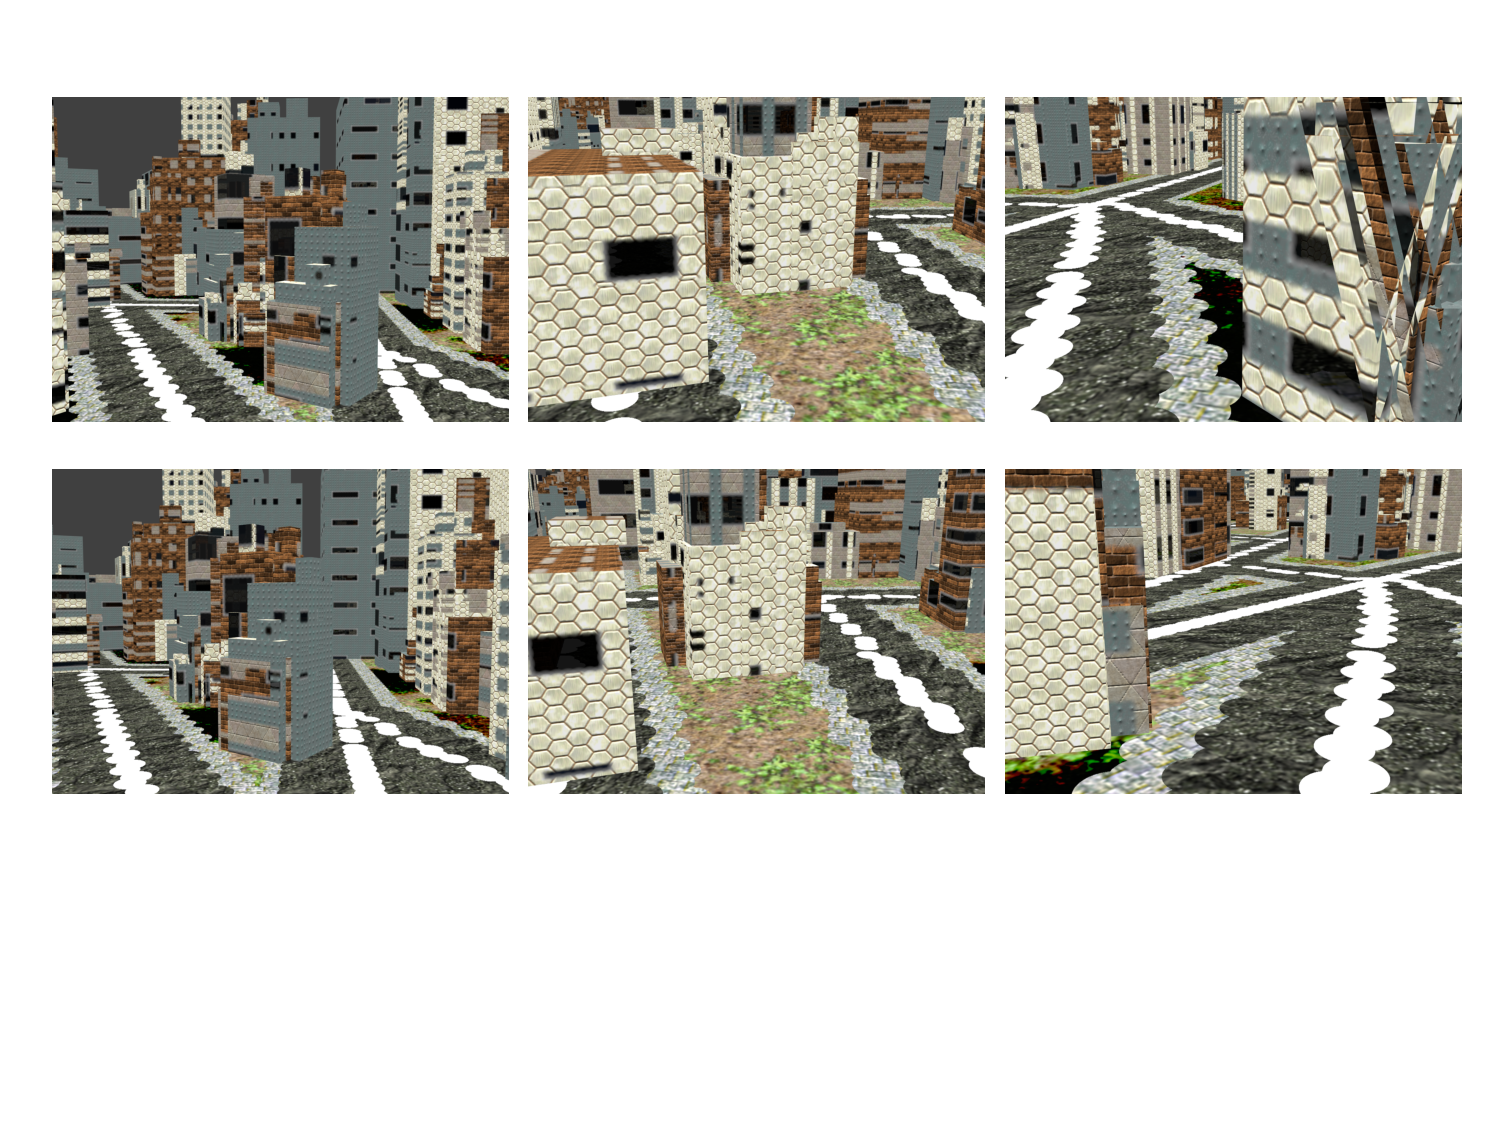
\includegraphics[width=0.95\columnwidth]{testPicture}
\caption{\label{fig:gatheredImage}Gathered image from Blender}
\end{center}
\end{figure}
We used an open source 3-D modeling software called Blender to generate a city
view for our simulation in this paper~\cite{Blender}.
Figure~\ref{fig:cityView}
Figure~\ref{fig:gatheredImage}
\input{Conclusion}

\bibliographystyle{IEEEtran}
\bibliography{reference}

\end{document} 